\section{Datenflussdiagramm}
Abschließend soll der Datenfluss innerhalb des Programms mithilfe von Abb. 6.1 genauer betrachtet werden.

\begin{figure}[h!]
	\centering
	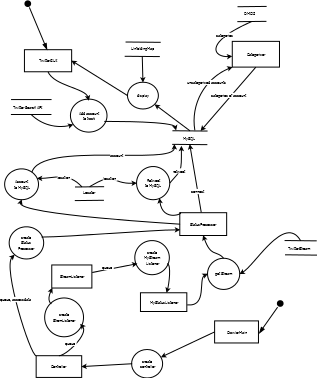
\includegraphics[width=\textwidth,height=\textheight,keepaspectratio=true]{dia/datenflussdiagramm}
	\caption{Datenflussdiagramm des gesamten Systems}
	\label{fig:datenflussdiagramm}
\end{figure}
Der Datenfluss beginnt in der Klasse CrawlerMain, in der die main-Methode gestartet wird. Zuerst fließen dort Zugangsdaten der Datenbank an ein Controller Objekt, welche für seine Erzeugung notwendig sind. \\
Ist dies abgeschlossen werden mehrere StatusProssesor Objekte erzeugt denen jeweils die Queue, in der später die zu verarbeitenden Tweets enthalten sein werden, und Zugangsdaten für die Datenbank übergeben. Diese StatusProcessor Objekte verbinden sich anschließend mit Hilfe der zuvor erhaltenen Zugangsdaten mit der Datenbank. Zeitgleich wird ein StreamListener Objekt erzeugt dem wiederum die vorhin beschriebene Queue übergeben wird. Sobald diese Initialisierung abgeschlossen ist erzeugt das StreamListener-Objekt ein MyStatusListener, dem es wieder die Queue mitliefert. Sobald dies geschehen ist beginnt der MyStatusListener Daten aus dem TwitterStream auszulesen und sie in die Queue zu schreiben, die der StatusProcessor permanent bearbeitet. Solche Tweet-Objekte fließen also durch die Queue zu einer der StatusProcessor Instanzen. \\
Sobald ein StatusProcessor Objekt erkennt, dass der gerade in Bearbeitung befindliche Tweet von einem verifizierten Account kommt, wird der Account mit Hilfe der Daten, die  der Lokalisierer liefert (dieser benutzt einen Web-Lokalisierungsdienst), in die Datenbank geladen. Stellt der StatusProcessor fest, dass es ein Retweet war, wird er zusammen mit den Daten aus dem Lokalisierer in die Datenbank geladen.\\
Sobald in der Datenbank Einträge vorhanden sind beginnt der Kategorisierer nach noch unkategorisierten Accounts zu suchen. Findet er solche, bekommt er die Accountdaten von der Datenbank und bestimmt mit Hilfe der DMOZ-Datenbank passende Kategorien. Diese werden dann in der Datenbank dem jeweiligen Account hinzugefügt.\\
Die in der Datenbank vorhandenen Daten können dann auf der TwitterGUI visualisiert werden. Dazu fließen die entsprechenden aufgearbeiteten Daten zusammen mit den notwendigen Daten für die UnfoldingMap-Darstellung zur GUI. Werden nun in der GUI zusätzliche Accounts zum Tracken angegeben, werden diese mit Hilfe der Twitter Search API an die Datenbank gesendet und der Kreislauf wird geschlossen.\\
Die TwitterGUI ist somit ein zweiter Startpunkt für den Datenfluss.	
	%end{description}
